%==============================================================================
%  RehabSense — ESP32-S3 Firmware Design  v2.0
%  CSE/EE 475 Embedded Systems Capstone + EE 542, Autumn 2026, Team 1
%  Compile with pdfLaTeX on Overleaf. Self-contained: no external image files.
%
%  Replaces "RehabSense Firmware Design — Prototype v0.1" (16 October 2026).
%  Normative source: RehabSense PRD v1.4 (22 October 2026), plus the four
%  decisions of 22 October recorded in §1.
%==============================================================================
\newcommand{\DocTitle}{RehabSense Firmware}
\newcommand{\DocSub}{ESP32-S3 firmware design, built to PRD v1.4}
\newcommand{\CourseLine}{CSE/EE 475 — Embedded Systems Capstone \,/\, EE 542 \quad\textbullet\quad
                         Team 1 \quad\textbullet\quad Autumn 2026}
\newcommand{\AuthorLine}{Aidan Goodman \quad\textbullet\quad firmware architecture}
\newcommand{\InstructorLine}{Instructor: Prof.\ Shwetak N.\ Patel \quad\textbullet\quad
                             TAs: Alex Ching, Guilin Hu}
%==============================================================================

\documentclass[11pt]{article}

% ---------- page ----------
\usepackage[letterpaper,margin=1in,headheight=14pt]{geometry}
\usepackage[T1]{fontenc}
\usepackage[utf8]{inputenc}
\IfFileExists{lmodern.sty}{\usepackage{lmodern}}{}
\IfFileExists{XCharter.sty}{\usepackage[scaled=1.0]{XCharter}}{}
\IfFileExists{FiraSans.sty}{\usepackage[sfdefault,scaled=0.92]{FiraSans}}{}
\IfFileExists{lmodern.sty}{\usepackage{microtype}}{\usepackage[expansion=false]{microtype}}

\usepackage{amsmath}
\usepackage{graphicx}
\usepackage{float}
\usepackage{array}
\usepackage{booktabs}
\usepackage{tabularx}
\usepackage{enumitem}
\usepackage[table]{xcolor}
\usepackage{titlesec}
\usepackage{fancyhdr}
\usepackage[most]{tcolorbox}
\usepackage{caption}
\usepackage{tikz}
\usetikzlibrary{arrows.meta,positioning,decorations.pathmorphing,shapes.geometric,calc,fit,backgrounds}
\usepackage[hidelinks]{hyperref}

% ---------- palette (shared with the PRD) ----------
\definecolor{ink}{HTML}{1C1C1C}
\definecolor{marker}{HTML}{E4572E}
\definecolor{annot}{HTML}{2E5EAA}
\definecolor{paper}{HTML}{FAF7F2}
\definecolor{rule}{HTML}{D8D2C8}
\definecolor{soft}{HTML}{6E6A64}
\definecolor{limb}{HTML}{DAD4CA}
\definecolor{good}{HTML}{2F7A52}
\definecolor{bad}{HTML}{A8322D}

\color{ink}

% ---------- headings ----------
\titleformat{\section}{\normalfont\large\bfseries\color{ink}}{\color{marker}\thesection}{0.8em}{}
\titlespacing*{\section}{0pt}{1.6em}{0.6em}
\titleformat{\subsection}{\normalfont\normalsize\bfseries\color{ink}}{\color{soft}\thesubsection}{0.7em}{}
\titlespacing*{\subsection}{0pt}{1.2em}{0.4em}
\titleformat{\subsubsection}[runin]{\normalfont\bfseries\color{ink}}{}{0pt}{}[.\hspace{0.4em}]

\setlist[itemize]{leftmargin=1.2em,itemsep=2pt,topsep=4pt}
\setlist[enumerate]{leftmargin=1.4em,itemsep=2pt,topsep=4pt}

\pagestyle{fancy}\fancyhf{}
\renewcommand{\headrulewidth}{0.4pt}
\fancyhead[L]{\small\color{soft}\DocTitle\ — Firmware Design v2.0}
\fancyhead[R]{\small\color{soft}\thepage}

\captionsetup{font=small,labelfont={bf,color=soft},textfont=it,width=0.9\linewidth}

% ---------- callout boxes ----------
\newtcolorbox{callout}[1][]{
  enhanced, breakable, colback=paper, colframe=rule, boxrule=0.6pt,
  arc=2pt, left=10pt, right=10pt, top=8pt, bottom=8pt, #1}

\newtcolorbox{phasebox}[1]{
  enhanced, breakable, colback=marker!6, colframe=marker, boxrule=1pt, arc=2pt,
  left=10pt,right=10pt,top=8pt,bottom=8pt,
  fonttitle=\bfseries\sffamily, title={#1}, coltitle=white, colbacktitle=marker}

\newtcolorbox{plainbox}{
  enhanced, breakable, colback=white, colframe=ink, boxrule=1pt, arc=2pt,
  left=10pt,right=10pt,top=8pt,bottom=8pt}

% ---------- status markers ----------
\newcommand{\built}{{\sffamily\scriptsize\color{good}\textbf{[built]}}\ }
\newcommand{\inpart}{{\sffamily\scriptsize\color{marker}\textbf{[partial]}}\ }
\newcommand{\todo}{{\sffamily\scriptsize\color{bad}\textbf{[hardware]}}\ }
\newcommand{\tested}{{\sffamily\scriptsize\color{annot}\textbf{[tested]}}\ }

\newcommand{\mY}{{\color{good}$\bullet$}}
\newcommand{\mP}{{\color{marker}$\circ$}}
\newcommand{\mN}{{\color{bad}$\times$}}

% Long \texttt identifiers are unbreakable; prefer loose lines to overfull ones.
\emergencystretch=3em
\hbadness=10000
\sloppy

% ---------- tikz styles ----------
\tikzset{
  lead/.style  ={line width=0.7pt, color=annot, -{Stealth[length=4pt]}},
  note/.style  ={font=\sffamily\scriptsize, color=annot, align=left, inner sep=1.5pt},
  flow/.style  ={-{Stealth[length=5pt]}, line width=0.9pt, color=ink},
  st/.style    ={draw=marker, line width=1.3pt, rounded corners=3pt, fill=marker!6,
                 align=center, inner sep=4pt, font=\sffamily\scriptsize, minimum width=22mm},
  stg/.style   ={draw=good, line width=1.3pt, rounded corners=3pt, fill=good!6,
                 align=center, inner sep=4pt, font=\sffamily\scriptsize, minimum width=22mm},
  blk/.style   ={draw=ink, line width=0.9pt, rounded corners=2pt, fill=white,
                 align=center, inner sep=4pt, font=\sffamily\scriptsize, minimum height=9mm},
}

\begin{document}

%==============================================================================
\begin{center}
{\LARGE\bfseries \DocTitle}\\[2pt]
{\large\color{soft} \DocSub}\\[10pt]
{\small \CourseLine}\\[2pt]
{\small \AuthorLine}\\[2pt]
{\small\color{soft} \InstructorLine}\\[2pt]
{\small\color{soft} Firmware design v2.0 \quad\textbullet\quad October 22, 2026 \quad\textbullet\quad
replaces Prototype v0.1 of 16 October}
\end{center}
\vspace{4pt}
{\color{rule}\hrule height 1pt}
\vspace{10pt}

%==============================================================================
\section{Summary}

This document specifies the RehabSense firmware and the interface contract
between the firmware and the Python host client. It replaces \emph{Prototype
v0.1} of 16 October in full, and it describes firmware that now exists:
7{,}701 lines of C in \texttt{main/}, built to PRD v1.4 and exercised by five
test suites that all pass.

\begin{callout}
\textbf{PRD v1.4 is normative.} Where this document and the PRD describe the
same behaviour, the PRD's description governs, and this document's job is to
say how that behaviour is realised on an ESP32-S3 --- which task owns it,
which register, which constant, which frame.

\medskip
\textbf{Four decisions of 22 October supersede the PRD} and are built as
stated here:

\smallskip
\begin{enumerate}
\item \textbf{One EMG channel for the prototype.} A single MyoWare 2.0 on the
biceps: two electrodes on the muscle belly about 20\,mm apart, plus one
reference on the bony elbow landmark --- three electrodes in all.
\item \textbf{ERM for the full production cycle.} The LRA is dropped. Every
reference to it is gone from the firmware and from this document.
\item \textbf{A soft click at 80\% of the target angle} --- PRD \S11.2 left
this open; it is now built as a seventh haptic pattern.
\item \textbf{Fatigue advises and does not stop the session} --- the other
open item in PRD \S11.2, now settled the same way.
\end{enumerate}
\end{callout}

\paragraph{What the single channel costs.} Co-contraction is a quarter of the
PRD \S5.5 score and needs an antagonist envelope, which one sensor on the
biceps does not provide. The component is therefore weighted zero and the
score normalises by the weights in force, so the three remaining components
take a third each rather than the best achievable score being capped at 75.
Calibration loses its triceps step, and the donning check loses its ability to
say \emph{the sleeve is on backwards} --- it can still catch a dead or
misplaced electrode, which \S10.1 explains. Everything that needs a second
channel is guarded on \texttt{EMG\_N\_CHANNELS} rather than deleted, so the
custom PCB's two-channel front end is a change of one constant.

\paragraph{Repository state.} \texttt{cse475/firmware}: an ESP-IDF project.
Six new files, thirty modified. The host client is 11 Python files in
\texttt{firmware/host}, updated in lockstep so that the two sides cannot
disagree about a byte.

\medskip
\noindent
Status markers below: \built\ built and exercised \quad
\inpart\ partly built \quad \todo\ waiting on hardware.

%==============================================================================
\section{What changed, and why it matters}

\subsection{PRD critical features}

\begin{table}[H]
\centering\small
\begin{tabularx}{\linewidth}{@{}p{48mm} c X@{}}
\toprule
\textbf{PRD \S3.2 critical feature} & & \textbf{State} \\
\midrule
Single-channel sEMG acquisition & \mY & Continuous DMA, 2\,kSPS \\
Dual-IMU elbow angle & \mY & Madgwick per sensor, relative rotation about the calibrated flexion axis \\
On-device repetition detection & \mY & Gated on biceps activation; counted on the return \\
On-device grading, 0--100 & \mY & Range, tempo and smoothness, equally weighted \\
Compensation detection & \mY & Shoulder at $20^{\circ}$, trunk as true common mode, momentum \\
Haptic feedback, three outcomes & \mY & Clean, flagged, set complete \\
Fault and rest cues & \mY & Both built; the fault cue plays before the mute \\
Non-overlapping cue playback & \mY & Single slot, priority, and fault preemption \\
Driver configuration self-test & \mY & Register read-back after every write \\
Host pattern test & \mY & Any of the seven patterns by id \\
BLE streaming and control & \mY & All twelve opcodes dispatched \\
Host application & \mY & \texttt{bleak} client, live plot, CSV log, MQTT \\
Calibration under 30\,s & \mY & Five steps, $\sim$16\,s of capture \\
Fatigue detection & \mY & Median-frequency regression; advises only \\
Battery operation, 2\,h & \mP & Sensing built; endurance is a hardware measurement \\
Custom PCB & --- & Hardware workstream \\
\bottomrule
\end{tabularx}
\end{table}

\subsection{The 29 October demonstration}

All seven items of PRD \S3.1 now work. The two that did not are the reason for
most of this revision.

\begin{table}[H]
\centering\small
\begin{tabularx}{\linewidth}{@{}p{6mm} X p{26mm}@{}}
\toprule
\textbf{\#} & \textbf{Demonstration item} & \textbf{State} \\
\midrule
1 & Sleeve, sensors, actuator, pod & Hardware workstream \\
2 & Don, check, calibrate, run a set with a haptic per repetition & \mY\ Works \\
3 & Shoulder elevation detected live, distinct haptic, lowered score & \mY\ Works \\
4 & A passively swung arm rejected --- no repetition starts & \mY\ \textbf{Now works} \\
5 & A fatiguing set, median frequency falling, rest cue firing & \mY\ Works \\
6 & Hold duration, repetition target, target angle changed live & \mY\ \textbf{Now works} \\
7 & Host showing live traces, per-repetition scores, summary & \mY\ Works \\
\bottomrule
\end{tabularx}
\end{table}

\subsection{The structural changes}

\begin{table}[H]
\centering\small
\begin{tabularx}{\linewidth}{@{}p{30mm} p{40mm} X@{}}
\toprule
\textbf{Subject} & \textbf{Was (v0.1)} & \textbf{Is now} \\
\midrule
Repetition start & Posture alone & \textbf{Biceps activation} and the start threshold (\S7.2) \\[3pt]
Where it is counted & At the top hold & On the \textbf{return}, after a confirming hold at extension \\[3pt]
Grading & Range 40, activation 25, smoothness 20, steadiness 15 & Range, tempo, smoothness --- equal weight; steadiness reported, not scored \\[3pt]
Smoothness & Normalised jerk & \textbf{Velocity-peak count}: one push scores 100 \\[3pt]
Muscle-on threshold & Fixed 0.15 \%MVC & Rest mean $+\,3\sigma$ on, $+\,2\sigma$ off, with confirmation windows \\[3pt]
Shoulder threshold & $15^{\circ}$ & $20^{\circ}$ \\[3pt]
Trunk lean & Inferred from upper-arm deviation & \textbf{Common-mode} rotation of both IMUs \\[3pt]
Calibration & Four phases, $\sim$95\,s & Five steps, $\sim$16\,s, individually repeatable \\[3pt]
Haptic patterns & Five, two of them invented & Seven, per PRD \S5.6 plus the soft click \\[3pt]
Set completion & Only on host \texttt{STOP} & At \texttt{rep\_target}, with the compound cue \\[3pt]
Host configuration & None & Fourteen TLV parameters (\S12.4) \\[3pt]
Opcodes dispatched & 8 of 12 & \textbf{12 of 12} \\
\bottomrule
\end{tabularx}
\end{table}

%==============================================================================
\section{Hardware configuration and pin map}

IMUs on SPI2, EMG on ADC1, and one short I\textsuperscript{2}C link to the
DRV2605L that carries traffic only at boot. No sensor data crosses a shared
bus.

\begin{table}[H]
\centering\small
\begin{tabularx}{\linewidth}{@{}p{33mm} p{23mm} p{19mm} X@{}}
\toprule
\textbf{Signal} & \textbf{Pin} & \textbf{Peripheral} & \textbf{Note} \\
\midrule
EMG (biceps) RAW & GPIO4 & ADC1\_CH3 & 12\,dB attenuation, $\sim$0--3.1\,V window \\
\textit{EMG B, Phase 2} & \textit{GPIO5} & \textit{ADC1\_CH4} & \textit{Unused on the prototype} \\
Battery sense & GPIO7 & ADC1\_CH6 & 2:1 divider, read while continuous mode is idle \\
SPI SCK / MOSI / MISO & GPIO12 / 11 / 13 & SPI2 (FSPI) & 10\,MHz, shared by both IMUs \\
CS, upper / forearm IMU & GPIO10 / 14 & GPIO out & \\
I\textsuperscript{2}C SDA / SCL & GPIO8 / 9 & I2C0 & DRV2605L only, 400\,kHz \\
Haptic PWM & GPIO6 & LEDC & DRV2605L IN/TRIG \\
Haptic enable & GPIO15 & GPIO out & Hard mute, bus-independent \\
Status LED & GPIO38 & RMT & On-board WS2812, DevKitC-1 v1.1 \\
User button & GPIO0 & GPIO in & On-board BOOT button \\
\bottomrule
\end{tabularx}
\end{table}

\noindent
Pins avoided: GPIO19--20 (USB D$-$/D$+$), GPIO26--32 (SPI flash), GPIO33--37
(octal PSRAM on the N8R8 module).

\paragraph{\built Electrode layout.} Three electrodes: two on the biceps
belly about 20\,mm apart and aligned with the muscle fibres, per SENIAM
guidance, and one reference on the bony landmark at the elbow. The custom PCB
adds the triceps pair and keeps the single shared reference, giving five.

\paragraph{\built Build configuration.} \texttt{sdkconfig.defaults} sets
\texttt{CONFIG\_SPIRAM\_MODE\_OCT=y} --- the single most common cause of an
N8R8 board reporting zero PSRAM --- along with
\texttt{CONFIG\_FREERTOS\_HZ=1000}, NimBLE only with a 247-byte preferred MTU,
Wi-Fi disabled, and a 5-second task watchdog. The 1\,kHz tick is what makes
the 70--80\,ms haptic gaps expressible; at the 100\,Hz default they could not
be timed at all.

\paragraph{\built BMI270 board configuration.} ADR jumper fully open (this is
what selects SPI, not cut to GND and not left at default),
I\textsuperscript{2}C pull-up jumpers cut, header pins mapped
SCL$\rightarrow$SCK, SDA$\rightarrow$PICO, ADR$\rightarrow$POCI,
CS$\rightarrow$CS. The device powers up in I\textsuperscript{2}C mode
regardless; the driver performs a dummy read of register \texttt{0x00} and
lets CSB rise, and that edge latches SPI mode.

\subsection{Sampling rates}

\begin{table}[H]
\centering\small
\begin{tabularx}{\linewidth}{@{}p{26mm} p{30mm} X@{}}
\toprule
\textbf{Stream} & \textbf{Rate} & \textbf{Note} \\
\midrule
EMG & 2\,kSPS & 1 channel; MyoWare RAW carries content to $\sim$500\,Hz \\
IMU & 100\,Hz per sensor & Accelerometer and gyroscope, both IMUs \\
Analysis & 50\,Hz & Hold timers and compensation confirmation need this \\
Feature frames on air & 20\,Hz & All a live plot requires [PRD \S12] \\
\bottomrule
\end{tabularx}
\end{table}

\noindent
\built The two feature rates are now separate: analysis at 50\,Hz,
transmission decimated to 20\,Hz. The saved bandwidth belongs to the raw
stream, which is busiest exactly when tuning sessions need it.

%==============================================================================
\section{EMG acquisition and signal chain}

The acquisition layer is written against an abstract interface, so the
prototype runs on the ESP32's internal ADC and the custom PCB runs on the
ADS131M02 with no change above the driver. \built Both backends are declared
and the switch is a single assignment at initialisation; the ADS131M02
implementation is a stub that fails loudly, which is correct for a board that
does not exist yet.

\paragraph{\built Internal ADC configuration.} Continuous DMA mode, not
one-shot. One-shot sampling from a timer callback produces jitter that smears
the spectrum, which is exactly the measurement fatigue detection depends on
--- PRD \S5.8 makes this a load-bearing choice. \texttt{adc\_continuous} on
ADC1, \texttt{ADC\_ATTEN\_DB\_12}, curve-fitting calibration, and a
conversion-done callback that fills 64 samples and posts to the DSP task by
queue.

\subsection{\built DSP chain}

Run in order on the raw stream at 2\,kSPS, using ESP-DSP
(\texttt{dsps\_biquad\_f32}, \texttt{dsps\_fft2r\_fc32}).

\begin{enumerate}
\item \textbf{High-pass, 20\,Hz, 2nd-order Butterworth.} Electrode half-cell
drift and motion artefact, and incidentally the internal ADC's offset error.
\item \textbf{Low-pass, 450\,Hz, 2nd-order Butterworth.}
\item \textbf{Notch, 60\,Hz, $Q \approx 30$.} A 180\,Hz harmonic notch sits
behind a compile-time flag.
\item \textbf{Clip detection.} Samples within 1\% of either rail, reported in
telemetry so front-end gain is set against a counter rather than by eye.
\item \textbf{Rectify and smooth.} Moving RMS over 150\,ms, decimated to 50\,Hz.
\item \textbf{Normalise.} Zeroed below the rest floor, then scaled so the
calibrated maximum reads 1.0.
\item \textbf{Median frequency.} 512-sample Hann-windowed FFT with 50\%
overlap, computed only while the envelope shows real activation.
\end{enumerate}

\begin{callout}
\tested \textbf{Verified numerically.} \texttt{test/verify\_dsp.py} measures
the assembled chain against known signals: $-3$\,dB at both corners (0.707 at
20\,Hz and 450\,Hz), 0.000 gain at 60\,Hz, 0.998 at 100\,Hz. Median frequency
lands within 2.1\,Hz on pure tones at 80, 150 and 300\,Hz, and falls
monotonically as a synthetic spectrum shifts downward --- the fatigue
signature the whole feature depends on.
\end{callout}

\paragraph{\built Mains measurement, for free.} The contact check needs to
know how much 60\,Hz the leads are picking up. Rather than a second spectral
estimate, the chain taps either side of the notch: the power the notch removes
\emph{is} the mains pickup, because the notch is narrow enough to take
essentially nothing else. Two slow exponential averages and a ratio.

\subsection{\built Muscle activation detector}

PRD \S5.4 specifies the detector that gates repetition start, and it is not a
fixed threshold.

\begin{table}[H]
\centering\small
\begin{tabularx}{\linewidth}{@{}p{26mm} p{40mm} X@{}}
\toprule
\textbf{Transition} & \textbf{Condition} & \textbf{Confirmation} \\
\midrule
Activation on & Envelope above rest mean $+\,3\sigma$ & Sustained 50\,ms \\
Activation off & Envelope below rest mean $+\,2\sigma$ & Sustained 100\,ms \\
\bottomrule
\end{tabularx}
\end{table}

\noindent
Rest mean and $\sigma$ both come from calibration step 1, so the detector
adapts to each session's own noise floor. It lives in
\texttt{main/emg/activation.c}, its own translation unit, so the host test
build can link it without the biquad chain and the FFT.

\begin{callout}
\textbf{The hysteresis is not decoration, and neither is the unit conversion.}

\medskip
A single-threshold detector chatters at the boundary, and chatter on this
signal means repetitions starting and abandoning at random. The asymmetric
windows --- fast to assert, slow to release --- are what make the gate usable
on a real limb. \tested The suite drives 100 ticks of deliberate chatter
either side of the midpoint and sees zero transitions.

\medskip
The subtler trap is that calibration measures in raw RMS while everything
downstream sees a \emph{normalised} envelope: zeroed below rest $\times$ 1.5,
then scaled so the maximum reads 1.0. A threshold expressed in raw units that
is not put through the same transform lands somewhere else entirely.
\texttt{activation\_init()} applies it, and both sides read the multiplier
from one constant --- if those diverge, the muscle-on gate silently stops
meaning what calibration measured.

\medskip
A rest capture so quiet that $3\sigma$ falls below the floor the DSP already
zeroes would make the gate fire on any non-zero sample, which is the opposite
of gating. The threshold is floored just above zero, and a capture with no
usable $\sigma$ at all falls back to a fixed fraction of MVC and says so
through \texttt{using\_fallback} --- it never fails open, because failing open
restores exactly the behaviour this replaces.
\end{callout}

\subsection{\built Fatigue detection}

Median frequency is tracked as a linear regression across the set. Three
consecutive repetitions with slope below $-0.5$\,Hz per repetition raise the
flag and fire the rest cue once. A consistency guard requires each of the last
few repetitions to sit below the one before, so a single noisy estimate cannot
fire a cue at a patient.

\medskip
\noindent
\textbf{Fatigue advises; it does not stop the session.} The cue fires, the
event is reported, and what to do about it is the patient's and the
therapist's decision. A device that ended a set on its own reading of a
frequency trend would be overruling the person doing the exercise.

%==============================================================================
\section{IMU and elbow angle}

Elbow angle is the \emph{relative} orientation of the two BMI270s, never
either one's absolute heading. With no magnetometer, absolute yaw is
unobservable and drifts without bound.

\begin{table}[H]
\centering\small
\begin{tabularx}{\linewidth}{@{}p{34mm} p{30mm} X@{}}
\toprule
\textbf{Parameter} & \textbf{Value} & \textbf{Reason} \\
\midrule
Accelerometer range & $\pm4\,g$ & Curls stay well under $2\,g$ \\
Gyroscope range & $\pm500$\,dps & Margin over fast arm swing \\
Output data rate & 100\,Hz, both & Far above the $\sim$10\,Hz content of a curl \\
Power mode & Performance & Low-power duty cycling adds timing jitter \\
Madgwick $\beta$ & 0.08 & Tuning knob between drift and responsiveness \\
\bottomrule
\end{tabularx}
\end{table}

\paragraph{\built Bring-up hazard.} The BMI270 ships inert and needs an
$\sim$8\,kB configuration blob uploaded over SPI before it produces data at
all. A device that reads the correct chip ID but returns zeros is almost
always a failed upload. The init routine verifies
\texttt{INTERNAL\_STATUS}~$=$~\texttt{0x01} and the self-test fails explicitly
if it does not.

\subsection{\built From quaternions to a joint angle}

\begin{enumerate}
\item At the comfortable-straight reference pose, capture and store both
orientations: \texttt{q\_upper0}, \texttt{q\_fore0}.
\item Each sample, compute each sensor's orientation relative to its own
reference.
\item The relative rotation between those two is the joint rotation,
independent of how either sensor is mounted.
\item Extract the flexion component about the dominant rotation axis, which is
itself identified during the ROM sweep as the principal axis of the relative
rotation --- so sleeve alignment is never assumed.
\end{enumerate}

\subsection{\built Gyroscope bias}

New in this revision. Calibration step 1 captures per-axis bias for both
sensors, and \texttt{fusion\_update()} subtracts it before fusing. An
uncorrected bias of even a fraction of a degree per second integrates into a
visible angle error over a set, and it is the one error the patient cannot
see. Bias is accumulated inside \texttt{fusion.c}, because that is where the
raw samples arrive; calibration only ever sees derived values.

\subsection{\built Drift management}

\begin{itemize}
\item \textbf{Session re-zero.} The reference pose is recaptured at the start
of every session, resetting accumulated error to zero.
\item \textbf{Rest-phase re-anchor.} When both IMUs show angular velocity
below 3\,dps and acceleration within 0.05\,$g$ of $1\,g$ for more than
300\,ms, the filter re-anchors to gravity. The confirming hold guarantees this
once per repetition.
\end{itemize}

%==============================================================================
\section{Compensation detection}

All three compensations are observable from the two arm IMUs plus gravity, and
all are evaluated only \emph{during} a repetition. Compensation detected at
any point is latched and reported at the confirming hold, so feedback arrives
at one predictable moment rather than interrupting the movement.

\begin{table}[H]
\centering\small
\begin{tabularx}{\linewidth}{@{}p{24mm} X p{24mm}@{}}
\toprule
\textbf{Compensation} & \textbf{Signature} & \textbf{Threshold} \\
\midrule
Shoulder elevation & Upper-arm IMU rotated from its calibration pose & $>20^{\circ}$ \\[3pt]
Trunk lean & \textbf{Common-mode} rotation of both IMUs & $>10^{\circ}$ \\[3pt]
Arm swing & Upper-arm angular velocity, sustained & $>30^{\circ}/$s for 200\,ms \\[3pt]
Sudden jolt & Acceleration spike on either IMU & $>2.5\,g$ \\
\bottomrule
\end{tabularx}
\end{table}

\begin{callout}
\built \textbf{Trunk lean is now a measurement, not an inference --- and that
fixed a scoring bug.}

\medskip
Trunk lean used to be inferred from a moderate upper-arm deviation while the
elbow was nearly still. Because it triggered at $10^{\circ}$ and shoulder
elevation at $15^{\circ}$, and both tested the \emph{same quantity}, any
deviation past $15^{\circ}$ with a slow elbow set both flags and cost $-35$
instead of $-20$. Every staged shoulder-compensation repetition was biased
downward by an extra 15 points, and tuning grading weights against volunteer
data would have absorbed the error rather than revealing it.

\medskip
\texttt{fusion.c} now computes a true common-mode figure: the smaller of the
two sensors' deviations, gated on their rotation axes pointing the same way.
Trunk lean carries the whole arm, so both IMUs rotate together about nearly
one axis; a shoulder hike moves the upper arm while the forearm follows the
elbow instead, and the axes diverge. The two cannot collide.

\medskip
\tested Two cases pin it: a $30^{\circ}$ upper-arm deviation with no
common-mode component flags shoulder and \emph{not} trunk; a $14^{\circ}$
rotation shared by both sensors flags trunk.
\end{callout}

\paragraph{Wrist substitution} is not detectable with this sensor set. It
needs a third IMU on the hand, which PRD \S9 places out of scope.

%==============================================================================
\section{Repetition detection}

\subsection{\built The cycle}

A repetition begins when the biceps activates and the arm rises past the start
threshold, and is counted when the arm has returned below the finish threshold
and been held still there for \texttt{hold\_duration\_ms}.

Counting on the return makes the score cover the whole movement including the
eccentric phase, where a weak limb usually fails first. The confirming hold
supplies a stationary moment at a predictable point, which is what the haptic
and the gravity re-anchor both need: feedback is scheduled, not reactive.

\begin{figure}[H]
\centering
\resizebox{\linewidth}{!}{%
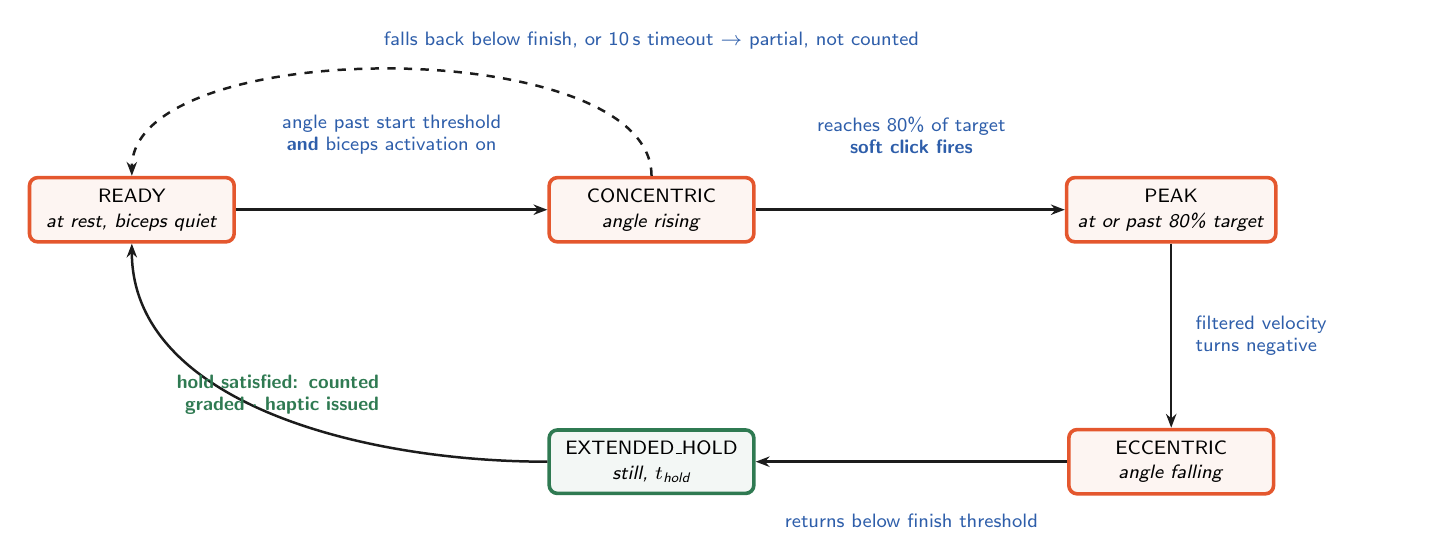
\begin{tikzpicture}[x=1cm,y=1cm]
\node[st,minimum width=26mm] (w)  at (0,0)       {READY\\[1pt]\textit{at rest, biceps quiet}};
\node[st,minimum width=26mm] (c)  at (6.6,0)     {CONCENTRIC\\[1pt]\textit{angle rising}};
\node[st,minimum width=26mm] (pk) at (13.2,0)    {PEAK\\[1pt]\textit{at or past 80\% target}};
\node[st,minimum width=26mm] (ec) at (13.2,-3.2) {ECCENTRIC\\[1pt]\textit{angle falling}};
\node[stg,minimum width=26mm] (xh) at (6.6,-3.2)  {EXTENDED\_HOLD\\[1pt]\textit{still, $t_{\text{hold}}$}};

\draw[flow] (w.east) -- (c.west);
\node[note,align=center,text width=36mm] at (3.3,0.95) {angle past start threshold\\\textbf{and} biceps activation on};

\draw[flow] (c.east) -- (pk.west);
\node[note,align=center,text width=32mm] at (9.9,0.95) {reaches 80\% of target\\\textbf{soft click fires}};

\draw[flow] (pk.south) -- (ec.north);
\node[note,align=left,anchor=west,text width=28mm] at (13.45,-1.6) {filtered velocity\\turns negative};

\draw[flow] (ec.west) -- (xh.east);
\node[note,align=center,text width=34mm] at (9.9,-3.95) {returns below finish threshold};

\draw[flow] (xh.west) .. controls +(-2.4,0) and +(0,-2.0) .. (w.south);
\node[note,align=right,anchor=east,text width=32mm,color=good] at (3.2,-2.35)
  {\textbf{hold satisfied: counted\\graded $\cdot$ haptic issued}};

\draw[flow,dashed] (c.north) .. controls +(0,1.8) and +(0,1.8) .. (w.north);
\node[note,align=center] at (6.6,2.15) {falls back below finish, or 10\,s timeout $\rightarrow$ partial, not counted};
\end{tikzpicture}}
\caption{The repetition cycle as built. Start is gated on biceps activation;
the count happens after the arm returns to the extended position and holds
still there.}
\end{figure}

\subsection{\built The activation gate}
\label{sec:gate}

\begin{callout}
This was the single largest gap in the firmware, and it is closed.

\medskip
PRD \S5.4 opens: ``A repetition begins when the biceps activates \emph{and}
the arm rises past the start threshold.'' That conjunction is what allows a
passively swung arm to be rejected --- demonstration item 4, an acceptance
criterion in \S6, and the distinction on which the project's premise rests.

\medskip
The old gate took \texttt{fusion\_out\_t} only. The EMG envelope was not a
parameter and was not consulted anywhere on the path to a counted repetition;
activation entered the system exactly once, where it was summed for the
\emph{score}. An arm swung passively through a full range, biceps silent
throughout, satisfied every gate in turn and was \textbf{counted}.

\medskip
\texttt{rep\_cycle\_tick()} now runs the activation detector on every tick and
\texttt{READY} cannot be left without it. An arm that rises with the agonist
quiet produces \texttt{REP\_EVT\_PASSIVE\_SWING}: reported to the host, never
counted, and it arms nothing.

\medskip
\tested The suite drives five full-range, correctly-postured, correctly-timed
repetitions with the envelope held at zero. Nothing counts, nothing even
starts, and the passive-swing event is raised. A separate case confirms the
gate needs \emph{both}: a static contraction at rest starts nothing either.
\end{callout}

\subsection{\built Parameters}

All of the following are host-configurable at runtime (\S12.4) and take effect
from the next repetition.

\begin{table}[H]
\centering\small
\begin{tabularx}{\linewidth}{@{}p{38mm} p{25mm} X@{}}
\toprule
\textbf{Parameter} & \textbf{Default} & \textbf{Basis} \\
\midrule
\texttt{target\_angle} & $110^{\circ}$ & Therapist-set. Volunteers peaked at $89$--$98^{\circ}$; the therapist starts patients lower \\
``Target reached'' & 80\% of target & The peak criterion, and where the soft click fires \\
\texttt{start\_angle} & $15^{\circ}$ & $20^{\circ}$ for limited extension \\
\texttt{finish\_angle} & $10^{\circ}$ & $5^{\circ}$ hysteresis below start \\
\texttt{hold\_duration\_ms} & 1000, 300--3000 & The primary tuning control: an impaired limb may not hold steadily for a full second \\
\texttt{hold\_velocity\_thresh} & $15^{\circ}/$s & A hold requires the limb stationary \\
Direction reversal & 5\,Hz low-passed velocity $<0$ & A fixed rate jitters at the top of a slow curl \\
\texttt{tempo\_min/max} & 1.5\,s, 3.5\,s & Start to finish, excluding the hold \\
Repetition timeout & 10\,s $\rightarrow$ partial & The 21 Oct session contained 16.6\,s and 24.7\,s ``repetitions'' \\
\texttt{rep\_target} & 20, range 1--50 & When the set-complete cue is issued \\
\bottomrule
\end{tabularx}
\end{table}

\noindent
\textbf{Thresholds are angles against the therapist's target}, not fractions
of measured ROM. The therapist prescribes what the patient \emph{should}
reach; measured ROM is what they currently can, and scoring against the latter
would hand full marks to a shrinking range.

\subsection{\built Behavioural rules}

Three rules hold regardless of parameters, and all three are implemented:

\begin{itemize}
\item Every completed repetition is counted and \emph{then} graded. Nothing is
silently discarded, because a counter that fails to advance gives the patient
no interpretable information.
\item A repetition flagged for compensation still counts toward the target.
Quality lives in the score, not in the counter.
\item Compensation detected at any point is latched and reported at the
confirming hold.
\end{itemize}

\paragraph{\built The start-posture gate is separate from the activation
gate.} A repetition begun with the upper arm already more than $15^{\circ}$
off its calibration attitude is refused rather than counted and penalised:
starting from a hike is a different error from developing one mid-curl, and
the patient can fix it before they begin. \tested Pinned by its own case.

%==============================================================================
\section{Grading}

Each repetition receives a score from 0 to 100. The patient receives only a
pass/fail distinction, through the choice of haptic pattern; the number is
shown in the application.

\begin{table}[H]
\centering\small
\begin{tabularx}{\linewidth}{@{}p{30mm} p{16mm} X@{}}
\toprule
\textbf{Component} & \textbf{Weight} & \textbf{Measure} \\
\midrule
Range of motion & 1/3 & Peak angle divided by the therapist's target angle \\[3pt]
Tempo & 1/3 & Start threshold to finish threshold, against the window \\[3pt]
Smoothness & 1/3 & Velocity peaks above 10\% of this repetition's peak velocity; one push scores 100 \\[3pt]
\textit{Co-contraction} & \textit{0} & \textit{Needs the second channel; Phase 2} \\
\midrule
\multicolumn{3}{@{}l}{\textbf{Deductions, applied after the mean; clamped to 0--100}}\\
Shoulder compensation & $-20$ & Upper-arm IMU past $20^{\circ}$ from its calibration pose \\
Trunk lean & $-15$ & Common-mode rotation of both IMUs past $10^{\circ}$ \\
Momentum / arm swing & $-15$ & Upper-arm angular velocity past $30^{\circ}/$s for 200\,ms \\
\bottomrule
\end{tabularx}
\end{table}

\noindent
Steadiness during the confirming hold is computed and \emph{reported} but
carries zero weight by default, per PRD \S5.5. It is available as an optional
fifth component by giving it a weight from the host.

\begin{callout}
\built \textbf{The score normalises by the weights in force.} A host that
switches a component off --- or a build with one channel, where
co-contraction has nothing to measure --- redistributes that share across the
rest rather than capping the best achievable score below 100. Without this,
every patient on the prototype would score at most 75 for a perfect
repetition, and the number on the therapist's screen would mean something
different from the number in the specification. \tested A perfect repetition
scores 100 with tempo switched off.
\end{callout}

\subsection{\built Smoothness: counting pushes}

PRD \S5.5 specifies a velocity-peak count rather than a jerk metric, and the
reason is interpretability: ``this movement had four separate pushes'' means
something to a therapist in a way that a normalised jerk figure does not.

Peaks are detected on a 5\,Hz low-passed velocity so that sensor noise does
not read as a correction the patient made, and their magnitudes are stored so
the 10\% threshold can be applied at the end, once the repetition's own peak
is known.

\medskip
\noindent
Counting peaks is also naturally scale-free, which matters more than it
sounds. \tested An unnormalised jerk metric --- the thing v0.1 shipped ---
handed a better score to anyone who simply moved slower, rewarding exactly the
guarding behaviour this device exists to discourage. The suite pins the fix
from both ends: a smooth curl at 2.4\,s and the same shape at 3.2\,s register
the identical peak count, and a four-push curl over the same range registers
more.

\subsection{\built Tempo}

Full credit inside the prescribed window, falling off linearly over one
window-width either side, so a repetition just outside is marked down rather
than zeroed. Both directions matter: too fast is momentum, too slow is usually
guarding or a stall mid-range.

\medskip
\noindent
Tempo is measured start threshold to finish threshold and \emph{excludes} the
confirming hold, which is why counting on the return matters --- the whole
excursion is inside the measurement.

%==============================================================================
\section{Haptics}

Feedback is delivered by an Adafruit 1201 ERM at the end of the confirming
hold, when the patient is stationary.

\subsection{\built Drive path}

An ERM's vibration frequency is coupled to its amplitude, so ``stronger'' also
means ``faster'' and cannot carry independent meaning. Every pattern is
therefore distinguished by \textbf{rhythm} --- pulse count, width and gap ---
and the six result cues play at one consistent amplitude, which is also easier
for a patient to learn than a set of intensity gradations.

\paragraph{Power-up sequence.} Reset the DRV2605L; leave standby; select ERM
drive (\texttt{N\_ERM\_LRA}~$=0$ in Feedback Control, \texttt{0x1A}); set the
rated voltage and overdrive clamp; run auto-calibration; store the results in
NVS; switch the mode register to PWM input; then read back every configured
register. A mismatch fails the self-test before the session begins. If
auto-calibration fails, the driver falls back to the stored calibration; if
none exists, initialisation fails rather than running with unknown drive
parameters.

\paragraph{\built PWM drive.} LEDC at 20\,kHz, 10-bit, with 50\% duty as zero
drive and deviation from 50\% setting amplitude. The output is held at zero
drive before the chip is switched into PWM mode, so the actuator cannot twitch
during configuration.

\paragraph{\built Onset.} Each pulse opens with a 20\,ms overdrive kick.
Without it an ERM's onset is soft and the pulse reads as a fade rather than a
tap --- the difference between a reward signal and a vague buzz. Active
braking through the driver is what makes 60\,ms gaps workable; without a
driver IC the floor would be $\sim$120\,ms, and the shortest gap any pattern
asks for is 70\,ms.

\paragraph{\todo Actuator limits.} \texttt{ERM\_RATED\_VOLTAGE\_V}~$=3.0$ and
\texttt{ERM\_OVERDRIVE\_CLAMP\_V}~$=3.3$ are starting values for a 2--5\,V
part. Confirm against the Adafruit 1201 datasheet during bring-up: wrong
values here produce a weak or buzzy actuator.

\subsection{\built The seven patterns}

\begin{table}[H]
\centering\small
\begin{tabularx}{\linewidth}{@{}p{34mm} p{46mm} X@{}}
\toprule
\textbf{Event} & \textbf{Pattern} & \textbf{Interpretation} \\
\midrule
Repetition counted, clean & One 100\,ms click & Met the form, range and tempo criteria \\[3pt]
Repetition counted, flagged & Three 80\,ms pulses, 80\,ms gaps & Counted, but incomplete range, outside the tempo window, or compensation \\[3pt]
Final repetition of the set & Two 70\,ms pulses with 70\,ms gaps, then one 500\,ms pulse & The repetition target has been reached \\[3pt]
Rest now & One 1000\,ms ramp up and down & Fatigue flag raised \\[3pt]
Fault & Two 300\,ms pulses, 300\,ms apart & Contact lost, sensor fault, or low battery \\[3pt]
Button press & One 40\,ms tick & Confirms every press \\[3pt]
\textbf{80\% of target} & One 30\,ms click at reduced level & \textbf{New:} you may begin the return \\
\bottomrule
\end{tabularx}
\end{table}

\begin{callout}
\textbf{The soft click is the only cue that fires mid-movement}, and it is
shaped so that it cannot be confused with a result.

\medskip
Everything else is delivered at a stationary moment and carries a verdict. The
soft click is a waypoint, so it is the shortest and lightest in the set, it
skips the overdrive kick that gives the others their snap, and it shares the
button tick's priority --- meaning it is \emph{dropped} rather than displacing
anything if a cue is already playing. A waypoint the patient misses costs
nothing; a result they miss costs the repetition.

\medskip
Two patterns from v0.1 are gone. \texttt{WRONG\_START} played at 50\%
amplitude, which broke the single-amplitude rule, and nagged every 2.5\,s
while a patient was trying to get into position; the app now shows that
instead. \texttt{BOOT\_OK} was two 100\,ms pulses 200\,ms apart, sitting in
the fault cue's rhythmic neighbourhood --- the same class of collision the PRD
records having had to fix once already. The status LED reports a successful
boot.
\end{callout}

\paragraph{\built Set completion.} On the repetition that reaches
\texttt{rep\_target}, a \emph{compound} pattern plays the per-repetition
result, a 300\,ms gap, then the set-complete cue, so the patient receives both
the quality result and confirmation that the set is finished. It is one
request rather than two queued ones, because a single-slot scheduler would
drop the second.

\subsection{\built Scheduling}

\begin{table}[H]
\centering\small
\begin{tabularx}{\linewidth}{@{}p{52mm} X@{}}
\toprule
\textbf{Rule [PRD \S5.6]} & \textbf{Implementation} \\
\midrule
One cue plays at a time & Queue of depth 1; the task plays to completion before taking another \\
A new cue takes the pending slot only on higher priority & \texttt{haptic\_play()} peeks, compares, and resets only on a win \\
A fault preempts a playing cue and clears anything pending & A cancel flag checked between segments, and no delay runs longer than 10\,ms without checking it \\
A tick is dropped if any cue is playing & Dropped on \texttt{haptic\_is\_busy()} \\
Priority: tick $<$ result $<$ set complete and rest $<$ fault & As stated. Clean and flagged share a rank: they are one class, and exactly one is issued per repetition \\
\bottomrule
\end{tabularx}
\end{table}

\noindent
\built \textbf{Fault preemption is the rule that needed real work.} Pattern
playback used to run to completion through \texttt{vTaskDelay} with nothing
able to interrupt it. Delays are now sliced, so a fault reaches the actuator
within about 10\,ms however long the cue in flight was going to be.

\paragraph{\built The fault cue plays \emph{before} the mute.} PRD \S5.2:
haptics are muted through the enable pin only after the fault cue finishes,
``so the fault state cannot silence its own warning.'' The old
\texttt{sm\_fault()} muted first, which is right for a runaway motor and
exactly wrong for a lifted electrode, where the cue \emph{is} the information.
The distinction is now which fault code was raised:
\texttt{fault\_warrants\_cue()} in \texttt{rehab\_types.h} names the faults
the patient must be told about, and the mute is deferred 1\,s for those and
immediate for the rest. The deferral is a deadline checked in
\texttt{sm\_tick()}, not a sleep, so the analysis task is never blocked
waiting for a pattern to finish.

\subsection{Latency budget}

\begin{table}[H]
\centering\small
\begin{tabularx}{\linewidth}{@{}X p{24mm}@{}}
\toprule
\textbf{Stage} & \textbf{Worst case} \\
\midrule
\texttt{analysis} task period & 20\,ms \\
Queue post and haptic task wake & $<2$\,ms \\
LEDC duty update & $<1$\,ms \\
ERM onset to perceptible, with overdrive & $\sim$20\,ms \\
\midrule
\textbf{Total} & \textbf{$\sim$43\,ms} \\
\bottomrule
\end{tabularx}
\end{table}

\noindent
Within the PRD's 50\,ms budget, and measured from the completion of the
confirming hold rather than from a movement.

\paragraph{\inpart Timing exposure.} \texttt{CONFIG\_FREERTOS\_HZ=1000} gives
1\,ms resolution, so the specified widths are expressible and the PRD's 10\%
tolerance is met on a quiet system. The exposure is preemption rather than
resolution: the haptic task is pinned to core 0 alongside the NimBLE host, so
a radio event during a pattern can stretch a gap. A scope capture during
bring-up settles it; if it proves marginal, segment timing moves to a hardware
timer and the task only arms it.

%==============================================================================
\section{Calibration}
\label{sec:calib}

Calibration runs as a sequence of short, separately commanded steps, so a
failed step can be repeated on its own without restarting. \built Capture
totals about sixteen seconds on the single-channel prototype, against a Must
of ``under 30\,s'' in PRD \S3.2 --- down from roughly ninety-five.

\subsection{\built Donning check, step 0}

\begin{enumerate}
\item \textbf{Both IMUs respond}, with elbow motion present during a prompted
curl.
\item \textbf{The EMG channel shows life} --- envelope above the noise floor.
\item \textbf{No saturation.} A clipping channel makes every other measurement
untrustworthy, and clipping destroys the median-frequency estimate while
leaving the envelope looking plausible.
\item \textbf{Mains pickup within limits}, measured as the power the 60\,Hz
notch removes.
\item \textbf{Placement}, below.
\end{enumerate}

\begin{callout}
\textbf{What one channel costs the donning check.} The two-channel test is a
comparison: during a prompted curl the biceps envelope must exceed the
triceps, and if it does not, the sleeve is on backwards or the leads are
crossed --- and the device can say \emph{which}.

\medskip
With one sensor there is nothing to compare against, so that specific
diagnosis is no longer available and the firmware does not pretend otherwise.
What it checks instead is that the channel responds to the movement it is
supposed to measure: the envelope while the elbow is moving must exceed its
level while still by a clear factor. A pair on the muscle belly clears it
comfortably; a lifted, misplaced or dead electrode does not.

\medskip
That catches the common failures. It cannot distinguish ``on the wrong
muscle'' from ``on the right muscle but not contracting'', and the message
the patient sees says so rather than claiming more --- it asks them to check
the two electrodes and the reference, which is the action either case needs.
\end{callout}

\subsection{\built The steps}

\begin{table}[H]
\centering\small
\begin{tabularx}{\linewidth}{@{}p{20mm} p{9mm} p{34mm} X@{}}
\toprule
\textbf{Step} & \textbf{Time} & \textbf{Patient does} & \textbf{Captured, and pass condition} \\
\midrule
0. Contact & 4\,s & Sits; sleeve on; one prompted curl & Saturation, mains, IMU response, placement \\[3pt]
1. Rest & 5\,s & Arm relaxed at the side, completely still & EMG resting mean \emph{and $\sigma$}, and \emph{gyroscope bias}. Rejected if movement is detected \\[3pt]
2. Straight arm & 2\,s & Straightens \emph{as far as is comfortable} and holds still & The $0^{\circ}$ reference pose and both neutral quaternions. Rejected if not still \\[3pt]
3. Biceps maximum & $3 \times 3$\,s & Elbow at $\sim$90$^{\circ}$, pushes up against a table & 100\% reference, strongest 500\,ms window, best of three \\[3pt]
\textit{4. Triceps max} & --- & --- & \textit{Phase 2, with the second channel} \\[3pt]
5. Range sweep & 6\,s & Two slow, full-range curls & Flexion axis as the principal axis of the relative rotation; $\theta_{\min}$, $\theta_{\max}$; baseline median frequency \\
\bottomrule
\end{tabularx}
\end{table}

\subsection{\built Four things the protocol now does}

\begin{description}[leftmargin=0pt,style=unboxed,itemsep=5pt]

\item[\textcolor{marker}{``Comfortable straight'', not ``hanging down''.}] PRD
\S5.3 records the 21 October finding that step 2 must instruct \emph{comfortable}
straight: calibrating against a hyperextended pose caused returns to finish
$10$--$12^{\circ}$ short of the finish threshold, so repetitions did not
complete. This is a prompt string and a pose, and it is the difference between
a working session and one where nothing counts.

\item[\textcolor{marker}{Stillness gates on steps 1 and 2.}] The phases used
to accumulate unconditionally and never reject. Movement during the rest step
corrupts gyroscope bias and therefore the joint angle for the whole session,
with no obvious symptom --- which is precisely why a gate is needed rather
than a warning. A brief wobble is tolerated; sustained movement rejects the
step with a message naming the cause.

\item[\textcolor{marker}{$\sigma$ is captured and kept.}] The old code
accumulated \texttt{rest\_sum\_sq} faithfully for ten seconds and then never
read it --- only the mean reached the record. The $\sigma$ the activation
detector depends on was computed and thrown away. It is now a field in the
calibration record, which is why the record is at version 2.

\item[\textcolor{marker}{Steps are individually commanded.}]
\texttt{CMD\_START\_CALIBRATION} has always carried a step argument on the
wire, and the host has always tested re-running one step; the firmware
discarded it. It is now honoured. The step most likely to fail is a maximum
contraction on a paretic limb, which is also the one a patient least wants to
repeat four others to get back to.

\end{description}

\subsection{\built Maximum contraction on an impaired limb}

Maximal effort is inconsistent on a paretic limb, and a single poor attempt
mis-scales every subsequent measurement. All three mitigations from PRD \S5.3
are built: best of three attempts, each measured as the strongest 500\,ms
window rather than a single loudest sample; a plausibility floor that flags
\texttt{MVC\_UNRELIABLE} rather than silently accepting a maximum that barely
clears the noise; and a clinician-supplied value pushed from the host, written
to the calibration characteristic, which sets
\texttt{CALIB\_FLAG\_CLINICIAN\_OVERRIDE} and clears the unreliable flag. That
last path existed as a flag definition and nothing else.

\subsection{\built Persistence and the returning patient}

Results are written to NVS under a patient profile key. Steps 1, 2 and 5
re-run every session, since they reset gyroscope bias and IMU drift and absorb
day-to-day variation in sleeve placement; step 3 is reused from the stored
profile until it expires.

\begin{callout}
\built \textbf{The short path now actually runs.} Two one-line defects
combined to prevent it: \texttt{calib\_record\_t.timestamp} was read by the
staleness check and written nowhere, and \texttt{tick\_donning()} passed a
literal zero for the current epoch because the device had no wall clock. Every
stored profile therefore read as expired, and every patient went through the
full protocol every single session.

\medskip
The record is now stamped at save time, the epoch comes from
\texttt{CMD\_SET\_TIME}, and ``no host time yet'' is treated as \emph{unknown
age} rather than \emph{expired} --- the profile is still internally
consistent, and forcing a full recalibration because the phone has not spoken
yet is worse than using it.
\end{callout}

%==============================================================================
\section{Firmware state machine}

Seven states. The host drives transitions, but the device refuses to enter
\texttt{OPERATIONAL} until the donning check has passed and a calibration
profile exists --- the host cannot override that, because scoring against a
bad reference is worse than not scoring at all.

\begin{table}[H]
\centering\small
\begin{tabularx}{\linewidth}{@{}p{26mm} p{28mm} p{18mm} X@{}}
\toprule
\textbf{State} & \textbf{BLE} & \textbf{Buffering} & \textbf{Exits on} \\
\midrule
\texttt{OFF} & Off & --- & Power button \\
\texttt{BOOT / SELF\_TEST} & Advertising & --- & Self-test result \\
\texttt{STANDBY} & Connected, status & --- & \texttt{START}, or short press \\
\texttt{DONNING\_CHECK} & Status + envelope & --- & Check pass or fail \\
\texttt{CALIBRATION} & Status + step progress & --- & Protocol complete or abort \\
\texttt{OPERATIONAL} & Full stream & Tier 1 + tier 2 & \texttt{STOP}, \textbf{set complete}, or fault \\
\texttt{FAULT} & Status only, cause & Sealed, readable & Reset \\
\bottomrule
\end{tabularx}
\end{table}

\paragraph{\built Set completion ends the set.} Reaching \texttt{rep\_target}
seals the buffer, issues the compound cue, emits \texttt{SET\_COMPLETE} and
returns to \texttt{STANDBY} for the rest interval. Previously a set ended only
when the host sent \texttt{STOP}, and there was no \texttt{rep\_target}
anywhere in the firmware.

\paragraph{\built BLE dropout is not a state.} A device in
\texttt{OPERATIONAL} with no connection stays in \texttt{OPERATIONAL}:
acquisition, repetition detection, grading, haptics and tier-2 filling all
continue, and only the transmit task idles. The publishers return
\texttt{ESP\_ERR\_INVALID\_STATE} when nobody is subscribed and every caller
treats that as normal rather than as an error.

\subsection{\built Status indication}

\begin{table}[H]
\centering\small
\begin{tabularx}{\linewidth}{@{}p{40mm} p{26mm} X@{}}
\toprule
\textbf{State} & \textbf{Colour} & \textbf{Pattern} \\
\midrule
Idle, advertising & Blue & Slow blink \\
Connected & Blue & Solid \\
Calibrating & Amber & Pulsing \\
Session running & Green & Fast blink \\
Session running, link down & Green & Magenta blink every 2\,s \\
Battery below 15\% & Amber & Double blink every 2\,s \\
Fault & Red & Solid \\
\bottomrule
\end{tabularx}
\end{table}

\paragraph{\built Battery.} GPIO7 through a 2:1 divider. ADC1 runs in
continuous DMA mode for EMG during a session and a one-shot read cannot share
the unit, so the battery is sampled whenever acquisition is idle --- at boot,
in \texttt{STANDBY}, and between sets --- and the last reading is held during
a session. That is sufficient for the rule it serves: below 15\% the device
completes the current set, then stops and saves. The decision is taken at a
set boundary, which is exactly when a fresh reading is available.

%==============================================================================
\section{Buffering and data retention}

\subsection{The arithmetic}

\begin{table}[H]
\centering\small
\begin{tabularx}{\linewidth}{@{}X p{22mm} p{22mm}@{}}
\toprule
\textbf{Stream} & \textbf{Rate} & \textbf{Bytes/s} \\
\midrule
EMG raw, 1 ch $\times$ 2\,kSPS $\times$ int16 & 2\,kHz & 4{,}000 \\
IMU, $2 \times (3 \text{ accel} + 3 \text{ gyro}) \times$ int16 & 100\,Hz & 2{,}400 \\
Derived features and events & 20\,Hz & $\sim$160 \\
\midrule
\textbf{Total} & & \textbf{$\sim$6.6\,kB/s} \\
\bottomrule
\end{tabularx}
\end{table}

\noindent
About 396\,kB per minute on one channel, against 648\,kB on two. The tiering
is unchanged, and the margin is simply larger.

\subsection{\built Three tiers}

\textbf{Tier 0 --- DMA landing buffers.} Two 64-sample buffers ping-ponged by
the ADC driver, about 32\,ms each. Exists only to decouple the conversion
callback from the DSP task.

\textbf{Tier 1 --- live ring in internal SRAM, 8 seconds.} Feeds the DSP
windows, serves the BLE transmit queue, and absorbs short connection stalls
with no backfill machinery at all. Most real dropouts are sub-second and never
escalate past this tier.

\textbf{Tier 2 --- session store in PSRAM, 600 seconds.} Ten minutes of
full-rate raw data. Reset on \texttt{START}, sealed on \texttt{STOP}.
Allocated with \texttt{heap\_caps\_malloc(size, MALLOC\_CAP\_SPIRAM)} and
verified at boot rather than assumed.

\subsection{\built Recovery after a dropout}

Every frame carries a monotonic \texttt{uint32} sequence number that resets at
\texttt{START}. The host acknowledges the highest contiguous sequence it has
received; the device may release tier-2 storage below that mark but holds
everything above it. On reconnect the host reads the retained range from the
status characteristic and requests what it missed.

\begin{callout}
\built \textbf{The request half is now wired.}
\texttt{CMD\_REQUEST\_BACKFILL} had an opcode, a host-side builder and a
characteristic to notify on --- and no \texttt{case} in the firmware's
dispatch, so a host that asked for a replay got silence. This was a known gap
in v0.1 and it closed the last PRD \S6 acceptance criterion that could not be
run at all.

\medskip
A new \texttt{storage} task serves requests one chunk at a time, paced at a
chunk every 20\,ms, so catching up never stalls real-time data. If part of the
requested range has aged out, the device serves what remains and sets the gap
flag --- it never silently serves a short range as though it were complete,
because a host that trusts an incomplete range reconstructs a session that
never happened.
\end{callout}

%==============================================================================
\section{BLE interface}

This section is the boundary between the firmware and the host client.
Everything is little-endian, and every sample carries a timestamp from a
single monotonic device clock.

\subsection{\built Services and characteristics}

\begin{table}[H]
\centering\small
\begin{tabularx}{\linewidth}{@{}p{30mm} p{24mm} p{18mm} X@{}}
\toprule
\textbf{Characteristic} & \textbf{Short UUID} & \textbf{Properties} & \textbf{Carries} \\
\midrule
Control & \texttt{A5B10002} & Write & Commands from host to device \\
Raw stream & \texttt{A5B10003} & Notify & EMG and IMU sample frames \\
Events and features & \texttt{A5B10004} & Notify & Feature frames and async events \\
Device status & \texttt{A5B10005} & Read, Notify & State, battery, signal quality, sequence range \\
Backfill & \texttt{A5B10006} & Notify & Replayed frames after a dropout \\
Calibration record & \texttt{A5B10007} & Read, Write & The \texttt{calib\_record\_t} struct \\
\textbf{Configuration} & \texttt{A5B10008} & Read, Notify & \textbf{New:} serialised TLV (\S12.4) \\
\bottomrule
\end{tabularx}
\end{table}

\subsection{\built Frame formats}

All stream frames share a 14-byte header: \texttt{type} (uint8), \texttt{seq}
(uint32), \texttt{t\_us} (uint64), \texttt{n} (uint8).

\begin{table}[H]
\centering\small
\begin{tabularx}{\linewidth}{@{}p{20mm} X p{20mm} p{18mm} p{12mm}@{}}
\toprule
\textbf{Type} & \textbf{Contents} & \textbf{Batch} & \textbf{Rate} & \textbf{Bytes} \\
\midrule
\texttt{0x01} EMG & $n \times$ int16 per channel & 80 samples & 25 frames/s & 174 \\
\texttt{0x02} IMU & $n \times (2 \times 6 \times$ int16) & 6 samples & 16.7 frames/s & 158 \\
\texttt{0x03} Features & Envelope, MDF, angle, deviation, state, count, flags, activation & 1 & 20\,Hz & 40 \\
\texttt{0x04} Event & Event id plus payload & 1 & Async & $\le 32$ \\
\bottomrule
\end{tabularx}
\end{table}

\noindent
\built \textbf{The EMG batch derives from the channel count.} Each sample is
2\,B per channel, so 80 samples of one channel and 40 of two both come to
$14 + 160 = 174$\,B --- the frame is the same size whichever front end is
fitted, and the frame \emph{rate} falls out of it. A
\texttt{\_Static\_assert} pins it inside the 180-byte budget, which exists
because macOS caps ATT MTU at 185 and \texttt{bleak} does not expose a
portable MTU request.

\subsection{\built Control commands}

All twelve opcodes are now dispatched. Four were not: \texttt{SET\_CONFIG},
\texttt{GET\_CONFIG}, \texttt{SET\_TIME} and \texttt{REQUEST\_BACKFILL}.

\begin{table}[H]
\centering\small
\begin{tabularx}{\linewidth}{@{}p{12mm} p{42mm} X@{}}
\toprule
\textbf{Opcode} & \textbf{Command} & \textbf{Payload} \\
\midrule
\texttt{0x01} & \texttt{START\_SESSION} & exercise id (uint8) \\
\texttt{0x02} & \texttt{STOP\_SESSION} & --- \\
\texttt{0x03} & \texttt{START\_CALIBRATION} & step (uint8) --- now honoured \\
\texttt{0x04} & \texttt{ABORT\_CALIBRATION} & --- \\
\texttt{0x05} & \texttt{REQUEST\_RECALIBRATION} & --- \\
\texttt{0x06} & \texttt{ACK\_SEQ} & highest contiguous seq (uint32) \\
\texttt{0x07} & \texttt{REQUEST\_BACKFILL} & start, end (uint32 $\times$ 2) \\
\texttt{0x08} & \texttt{SET\_CONFIG} & TLV block (\S12.4) \\
\texttt{0x09} & \texttt{GET\_CONFIG} & --- \\
\texttt{0x0A} & \texttt{HAPTIC\_TEST} & pattern id (uint8) \\
\texttt{0x0B} & \texttt{SET\_TIME} & host epoch microseconds (uint64) \\
\texttt{0x0C} & \texttt{POWER\_OFF} & --- \\
\bottomrule
\end{tabularx}
\end{table}

\paragraph{\built The config opcode is no longer overloaded.} A write to the
\emph{calibration} characteristic used to be forwarded to the command callback
under \texttt{CMD\_SET\_CONFIG}. The two carry entirely different payloads,
and the moment a real TLV parser existed, a \texttt{calib\_record\_t} would
have been fed to it. Calibration writes now arrive under an internal opcode
that never appears on the wire.

\paragraph{\built Time synchronisation.} On connection the host sends
\texttt{SET\_TIME} with its own epoch; the device records the \emph{offset},
reports it in the status characteristic, and \textbf{never adjusts its own
clock}. Adjusting a sampling clock to match a phone would corrupt exactly the
timing the spectral analysis depends on --- the fatigue index is a frequency
measurement, and a frequency measured against a clock that jumps is not a
measurement.

\subsection{\built Runtime configuration}
\label{sec:config}

PRD \S5.9.1 requires every parameter below to be settable over BLE, changeable
during a session, effective from the next repetition, stored in NVS and read
back for confirmation. None of it existed; all of it does now, including the
tag vocabulary, which neither side had defined.

\begin{table}[H]
\centering\small
\begin{tabularx}{\linewidth}{@{}p{10mm} p{38mm} p{16mm} X@{}}
\toprule
\textbf{Tag} & \textbf{Parameter} & \textbf{Type} & \textbf{Default and range} \\
\midrule
\texttt{0x01} & \texttt{hold\_duration\_ms} & uint16 & 1000, 300--3000 \\
\texttt{0x02} & \texttt{hold\_velocity\_thresh} & float & $15^{\circ}/$s \\
\texttt{0x03} & \texttt{rep\_target} & uint8 & 20, 1--50 \\
\texttt{0x04} & \texttt{set\_count} & uint8 & 3 \\
\texttt{0x05} & \texttt{rest\_seconds} & uint16 & 60 \\
\texttt{0x06} & \texttt{target\_angle} & float & $110^{\circ}$ \\
\texttt{0x07} & \texttt{start\_angle} & float & $15^{\circ}$ \\
\texttt{0x08} & \texttt{finish\_angle} & float & $10^{\circ}$ \\
\texttt{0x09} & \texttt{tempo\_min}, \texttt{max} & float $\times$ 2 & 1.5\,s, 3.5\,s \\
\texttt{0x0A} & Compensation thresholds & float $\times$ 3 & $20^{\circ}$, $10^{\circ}$, $30^{\circ}/$s \\
\texttt{0x0B} & Grading weights & float $\times$ 5 & range, tempo, smoothness, co-contraction, steadiness \\
\texttt{0x0C} & Deductions & float $\times$ 3 & 20, 15, 15 \\
\texttt{0x0D} & \texttt{raw\_stream\_enable} & uint8 & On during tuning \\
\texttt{0x0E} & Exercise id, agonist channel & uint8 $\times$ 2 & 0, 0 \\
\bottomrule
\end{tabularx}
\end{table}

\begin{callout}
\textbf{Three properties of the TLV encoding earn their place.}

\medskip
\textbf{Unknown tags are skipped; wrong lengths are rejected.} A newer host
may send tags an older build has never heard of, and skipping lets the rest of
the block land. But a \emph{recognised} tag with the wrong length means the
two sides disagree about what it means, and guessing would write a plausible
wrong value into a live session.

\medskip
\textbf{Every value is clamped to a range the device can honour.} A
configuration that cannot produce a countable repetition is worse than a
rejected write, because it shows up as a device that has quietly stopped
counting rather than as an error. The finish threshold is forced below the
start threshold, since without hysteresis the cycle chatters between
\texttt{READY} and \texttt{CONCENTRIC}; the peak criterion is forced
reachable; and an all-zero weight vector restores the defaults rather than
scoring every repetition zero.

\medskip
\textbf{\texttt{GET\_CONFIG} returns the same block.} That is how the host
confirms a write took effect, and it is why the configuration has its own
readable characteristic rather than being inferred from behaviour.
\end{callout}

%==============================================================================
\section{Task architecture and timing}

\built The NimBLE host owns core 0. Everything latency-sensitive goes on core
1, where radio activity cannot preempt it.

\begin{table}[H]
\centering\small
\begin{tabularx}{\linewidth}{@{}p{24mm} p{8mm} p{10mm} p{20mm} p{10mm} X@{}}
\toprule
\textbf{Task} & \textbf{Core} & \textbf{Prio} & \textbf{Trigger} & \textbf{Stack} & \textbf{Job} \\
\midrule
ADC conv-done & 1 & ISR & 32\,ms DMA & --- & Hand the buffer to the DSP queue \\
\texttt{emg\_dsp} & 1 & 20 & Queue & 8\,kB & Biquads, envelope, FFT, clip count \\
\texttt{imu\_task} & 1 & 18 & 10\,ms timer & 4\,kB & Read both BMI270s, Madgwick \\
\texttt{analysis} & 1 & 16 & 20\,ms timer & 6\,kB & Angle, hold timers, cycle, compensation, grading \\
\texttt{haptic} & 0 & 22 & Queue & 2\,kB & Pattern playback as LEDC duty \\
\texttt{ble\_tx} & 0 & 12 & Queue & 6\,kB & Frame packing and notification \\
\texttt{storage} & 0 & 8 & Poll & 4\,kB & Tier-2 writes, backfill service \\
\texttt{housekeeping} & 0 & 5 & 1\,s timer & 3\,kB & Battery, status, LED, watchdog \\
\bottomrule
\end{tabularx}
\end{table}

\paragraph{\built Data flow.} ADC DMA to \texttt{emg\_dsp} by queue;
\texttt{emg\_dsp} and \texttt{imu\_task} publish into a shared, mutex-free
double-buffered state block that \texttt{analysis} reads at 50\,Hz.
\texttt{analysis} emits events into the haptic queue and the BLE queue
independently --- \textbf{the haptic path never waits on the BLE path}, which
is what keeps feedback working during a dropout. Queue depths are four frames;
an overrun sets a flag in the frame header rather than blocking the producer,
because dropping a sample and recording it is always better than stalling
acquisition.

\paragraph{\built Watchdog.} The task watchdog subscribes \texttt{emg\_dsp},
\texttt{imu\_task} and \texttt{analysis} with a 5-second timeout. A missed feed
drives the device into \texttt{FAULT}: haptics muted, acquisition stopped,
cause reported, LED red. The device does not silently reboot mid-set.

%==============================================================================
\section{Verification}

\subsection{\built What runs}

Five suites run on a laptop with no hardware, no radio and no ESP-IDF.
\tested All five pass.

\begin{table}[H]
\centering\small
\begin{tabularx}{\linewidth}{@{}p{34mm} X p{18mm}@{}}
\toprule
\textbf{Suite} & \textbf{Covers} & \textbf{Result} \\
\midrule
\texttt{test/test\_rep.c} & Compiles the real \texttt{rep\_cycle.c}, \texttt{grading.c} and \texttt{activation.c}; drives simulated angle and EMG traces & 16 scenarios pass \\
\texttt{test/verify\_dsp.py} & Filter response and the median-frequency estimator against known signals & All pass \\
\texttt{host/test\_protocol.py} & Wire format: every struct, every frame, every event, all twelve commands, the config TLV & All pass \\
\texttt{host/test\_grading.py} & The Python mirror of \texttt{grading.c} & All pass \\
\texttt{host/test\_sim\_session.py} & The host client against the device simulator & All pass \\
\bottomrule
\end{tabularx}
\end{table}

\subsection{\built What the repetition suite pins}

Eight scenarios became sixteen. The ones that matter most are the ones that
would otherwise fail silently:

\begin{itemize}
\item \textbf{Ten deliberate repetitions count as exactly ten} --- the
29 October acceptance gate, directly.
\item \textbf{A passive swing counts nothing and starts nothing}, and reports
itself (\S7.2).
\item \textbf{The gate needs both} muscle and movement; neither alone arms.
\item \textbf{A long hold at the top counts nothing}; the count follows the
return.
\item \textbf{Set completion fires exactly once}, at targets of 5 and 20.
\item \textbf{Tempo is measured and scored}, and a 9\,s repetition scores
below a 2.4\,s one.
\item \textbf{Smoothness counts pushes and does not reward slowness.}
\item \textbf{A shoulder hike does not also register as trunk lean}, and a
genuine common-mode rotation does.
\item \textbf{Host configuration takes effect} --- hold duration and target
angle both change the outcome.
\item \textbf{The activation detector does not chatter} across 100 ticks at
its own boundary.
\end{itemize}

\subsection{\built Closing the simulator gap}

\begin{callout}
v0.1's audit recorded a caution: the host suites test the host against
\texttt{rehab\_sim.py}, and the simulator was a \emph{more capable} device
than the real one --- it dispatched three opcodes the firmware did not. ``All
tests pass'' therefore did not establish that firmware and host interoperate.

\medskip
That gap is closed from both ends. The firmware dispatches all twelve opcodes,
and the simulator now implements the same repetition cycle, the same
activation detector, the same grading and the same configuration codec as the
device. Where the two could still drift --- struct layouts --- the layout is
pinned on both sides by arithmetic over \texttt{EMG\_N\_CHANNELS}, with a
\texttt{\_Static\_assert} in C and an assertion in Python.

\medskip
The caution has not disappeared, and it should not. A simulator is still not a
device. The first real interoperability evidence remains the bring-up gate:
60 seconds logged by the Python client with zero sequence gaps.
\end{callout}

%==============================================================================
\section{Defects fixed}
\label{sec:defects}

The nine defects the 22 October audit found are fixed. Two more were found
while fixing them, and both were wire-format bugs that only a real device
would have exposed.

\begin{table}[H]
\centering\small
\begin{tabularx}{\linewidth}{@{}p{40mm} X@{}}
\toprule
\textbf{Defect} & \textbf{Resolution} \\
\midrule
\texttt{timestamp} never written & Stamped at save time from the host epoch \\[3pt]
\texttt{is\_stale(\&rec, 0)} & Given the real epoch; unknown age no longer means expired \\[3pt]
Trunk and shoulder double-count & Trunk lean is now true common mode (\S6) \\[3pt]
\texttt{rest\_sum\_sq} discarded & $\sigma$ is stored in the record and drives the activation detector \\[3pt]
\texttt{CLINICIAN\_OVERRIDE} never set & Set by \texttt{calibration\_set\_record()} on a host write \\[3pt]
Calibration step argument ignored & Honoured; any step runs on its own \\[3pt]
Battery hard-coded to zero & Sampled while acquisition is idle \\[3pt]
\texttt{SET\_CONFIG} overloaded & Calibration writes use an internal opcode \\[3pt]
Tier-2 capacity misstated & Stated as the 600\,s the constant actually sets \\
\midrule
\multicolumn{2}{@{}l}{\textbf{Found during this work}}\\[3pt]
\texttt{device\_status\_t} layout mismatch & \textbf{The host expected 40 bytes with padding that the \texttt{packed} C struct does not have.} Every field after \texttt{battery\_mv} --- battery, sequence range, clip counters, repetition count and the clock offset --- would have been read from the wrong offset on real hardware. Both sides now derive the layout from one expression, and both assert it \\[3pt]
\texttt{features\_t} layout assumed two channels & Same class of problem, found the same way. Now derived from \texttt{EMG\_N\_CHANNELS}, including the compiler's internal pad byte \\
\bottomrule
\end{tabularx}
\end{table}

\begin{callout}
\textbf{Why the status-struct bug survived so long is the useful part.} The
host suites parse what the host builds, so a layout that is wrong in the same
way on both sides round-trips perfectly. It took comparing
\texttt{sizeof(device\_status\_t)} against \texttt{STATUS.size} --- a C
program and a Python expression, compared by hand --- to see it.

\medskip
That is now a build-time check rather than an act of attention: the C side
carries \texttt{\_Static\_assert} and the Python side an assertion, both over
the same arithmetic. A field added to one and forgotten on the other fails to
build.
\end{callout}

%==============================================================================
\section{What remains}

Everything outstanding now needs hardware, a decision, or volunteer data ---
there is no firmware work on the critical path for 29 October.

\begin{phasebox}{Needs the bench}
\begin{enumerate}
\item \textbf{Confirm the ERM's rated voltage and overdrive clamp} against the
Adafruit 1201 datasheet before the first auto-calibration. Wrong values give a
weak or buzzy actuator.
\item \textbf{Scope the haptic pattern timing} on the PWM line against the
10\% tolerance, with BLE active, to settle the core-0 preemption question
(\S9.4).
\item \textbf{Goniometer check} of the elbow angle at $0$, $45$, $90$ and
$135^{\circ}$, and tune Madgwick $\beta$ from the result.
\item \textbf{Set the front-end gain} against the clipping counter rather than
by eye, and confirm the counter reads zero at maximum effort.
\item \textbf{Blindfolded discrimination} of all seven patterns through
fabric.
\item \textbf{Two hours of battery operation}, and the low-battery behaviour
at the set boundary.
\end{enumerate}
\end{phasebox}

\begin{phasebox}{Needs volunteer data}
\begin{enumerate}
\item \textbf{Tune the grading weights and the tempo window.} Everything is
host-settable now, so this is a tuning session rather than a rebuild.
\item \textbf{Tune the compensation thresholds} with volunteers staging each
compensation deliberately.
\item \textbf{Check the activation thresholds} on a real limb --- in
particular how often \texttt{using\_fallback} fires, which would mean rest
captures are not yielding a usable $\sigma$.
\end{enumerate}
\end{phasebox}

\begin{phasebox}{Needs a decision}
\begin{enumerate}
\item \textbf{Cue blanking} (PRD \S5.6): suspend IMU and EMG analysis for the
duration of each cue? Nothing is implemented, and nothing should be until the
firmware and algorithms owners agree, because it changes scoring behaviour
around every cue. The soft click makes this slightly more pressing, since it
is the one cue that fires while the patient is moving.
\item \textbf{Repetition events to flash}, so they survive power loss
independently of the PSRAM session buffer (PRD \S5.9). The partition table
reserves space; nothing writes to it.
\end{enumerate}
\end{phasebox}

\paragraph{Phase 2, with the custom PCB.} Set \texttt{EMG\_N\_CHANNELS} to 2.
That restores the triceps channel, the co-contraction component at its PRD
weight, the triceps maximum as calibration step 4, and the two-channel
orientation test in the donning check. Every one of those paths is written and
guarded rather than deleted, and the frame layouts, the calibration record and
the status struct all derive their sizes from that constant.

%==============================================================================
\section{Design invariant}

Unchanged from v0.1, and this revision is the evidence for it:

\begin{plainbox}
Channel-to-muscle mapping, electrode sites, thresholds, hold durations and
scoring weights are \textbf{configuration}, not structure. Changing the
measured muscle pair or moving the electrodes touches a header file --- not
the acquisition, timing, transport or state machine layers.
\end{plainbox}

\noindent
This revision moved the actuator, halved the channel count, moved where a
repetition is counted, replaced the scoring model, replaced the muscle-on
detector, rebuilt the calibration protocol and added a runtime configuration
layer. The acquisition path, the DSP chain, the fusion layer, the buffering
tiers and the task architecture absorbed all of it without structural change.

\medskip
\noindent
The one place the invariant had to be \emph{enforced} rather than relied upon
is the channel count, which reaches into three wire formats. It is now a
single constant that both sides derive from, with assertions on both ends ---
which is what the invariant looks like when it is load-bearing rather than
aspirational.

\end{document}
